\documentclass{standalone}
\usepackage{tikz}
\usepackage{ctex,siunitx}
\setCJKmainfont{Noto Serif CJK SC}
\usepackage{tkz-euclide}
\usepackage{amsmath}
\usetikzlibrary{patterns, calc,3d}
\usetikzlibrary {decorations.pathmorphing,decorations.pathreplacing,decorations.shapes}
\begin{document}
\small
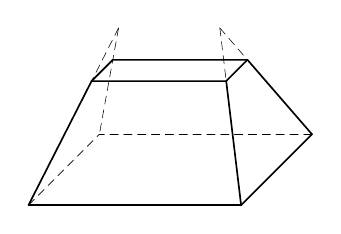
\begin{tikzpicture}[>=latex,scale=0.9]
  \tkzDefPoints{0/0/A,3/0/B,4/1/C,1/1/D,2.7/2.5/E}
  \tkzDefPointOnLine[pos=0.3](E,B)\tkzGetPoint{B'}
  \tkzDefPointOnLine[pos=0.3](E,C)\tkzGetPoint{C'}
  \tkzDefShiftPoint[B'](-1.9,0){A'}
  \tkzDefShiftPoint[C'](-1.9,0){D'}
  \tkzInterLL(A,A')(D,D')\tkzGetPoint{F}
  \tkzDrawSegments[semithick](A,B B,C B',C' A',B' A,A' C',D' D',A' B,B' C,C')
  \tkzDrawSegments[densely dashed](A,B B,C C,D E,B' E,C' A,D F,D F,A')
\end{tikzpicture}
\end{document}